% !TEX encoding = UTF-8
% !TEX program = pdflatex
% !TEX root = InformationRetrieval.tex
% !TEX spellcheck = it-IT

% 21 Ottobre 2016

%\section{Modello di reperimento}
%\subsection{Modello booleano}
%\subsubsection{Espressione della esigenza informativa}

\noindent Ad esempio con il nostro insieme di documento è possibile fare le seguenti query:

\begin{itemize}
	\item \textit{``pagine OR web''}: vengono forniti in risposta D1 e D3.
	\item \textit{``pagine AND web''}: solo il documento D1.
	\item \textit{``fasi AND web''}: nessun documento.
	\item \textit{``web AND NOT pagine''}: solo il documento D3. 	
\end{itemize}

\noindent Da notare che i documenti non vengono forniti con un ordinamento particolare perché la funzione di reperimento non calcola uno score dei documenti ma associa l'interrogazione al sotto-insieme di documenti che la rendono vera.

\subsubsection{Considerazioni sul modello booleano}

Il modello booleano è molto efficace in ambienti controllati e se l'utente è consapevole di come funziona il sistema e se sa quello che vuole. Magari se l'utente non è esperto può essere aiutato da un intermediario, che può essere un software o una persona.

Bisogna inoltre tenere conto che gli umanisti non conoscono la logica booleana e non sanno distinguere l'and dall'or.

Un altro problema di questo modello è legato alla dimensione dell'output, sulla quale non si ha controllo e può capitare sia di non avere risultati, che di averne troppi. Questo perché non ci sono misure di similarità/pesatura.

Il modello può inoltre essere esteso aggiungendo altri operatori, oltre a quelli booleani:

\begin{itemize}
	\item \textbf{operatori di prossimità}: per permettere la ricerca di frasi o di termini ad una certa distanza.
	\item \textbf{operatori di relazione}: $>, <, =, \leq, \ldots$.
	\item \textbf{operatori di troncamento dei descrittori}: per la ricerca utilizzando le radici dei termini.
\end{itemize}

\noindent Altri operatori possono essere quelli che fornisce Google: \url{https://support.google.com/websearch/answer/2466433?p=adv_operators\&hl=en\&rd=1}.

\subsection{Ordinamento dei risultati in base alla rilevanza}

Se il modello può fornire un ordinamento, quindi se si può effettuare il ranking dei documenti, si ha che i documenti formano una lista in cui a ciascun documento è assegnato un \textbf{rango} (o rank).

Il primo documento della lista ha un \textbf{rango alto} che corrisponde al \textbf{minimo valore intero di posizione nella lista} (ovvero al primo elemento della lista). L'ultimo documento della lista ha un \textbf{rango basso} che corrisponde al \textbf{massimo valore intero di posizione nella lista} (ovvero all'ultimo elemento della lista).

\subsection{Livello di coordinamento}

Il livello di coordinamento è un metodo e tecnica accessoria che può essere utilizzata per ordinare i documenti.
Più precisamente: il livello di coordinamento è una misura di quanto l'interrogazione è vera per un documento.

Il livello di coordinamento più semplice è quello \textbf{binario}, che vale 1 quando il documento in esame rende vera l'interrogazione e 0 in caso contrario.

\begin{figure}[ht]
	\centering
	\begin{minipage}[b]{0.45\linewidth}
		\centering
		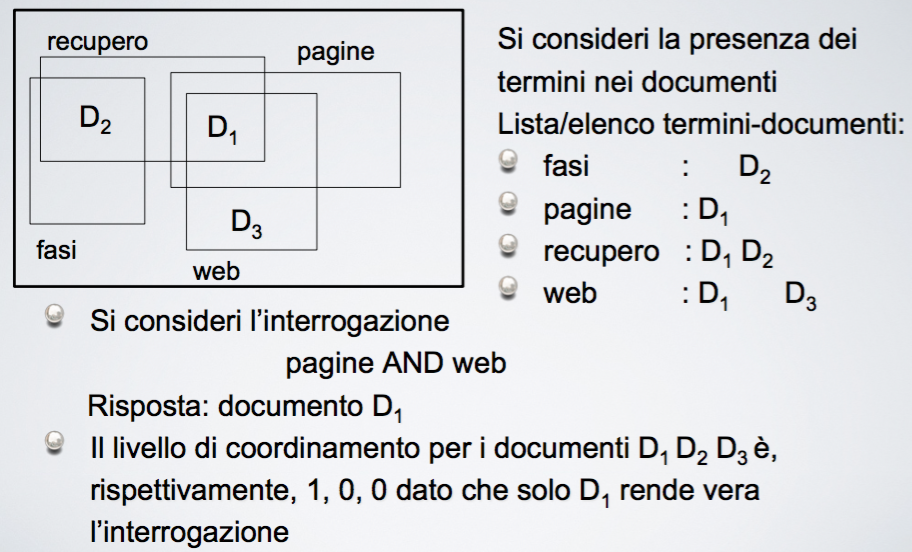
\includegraphics[width=0.7\linewidth]{images/l8-set-1}
		\caption{Livello di coordinamento con \textit{AND}}
		
	\end{minipage}
	\quad
	\begin{minipage}[b]{0.45\linewidth}
		\centering
		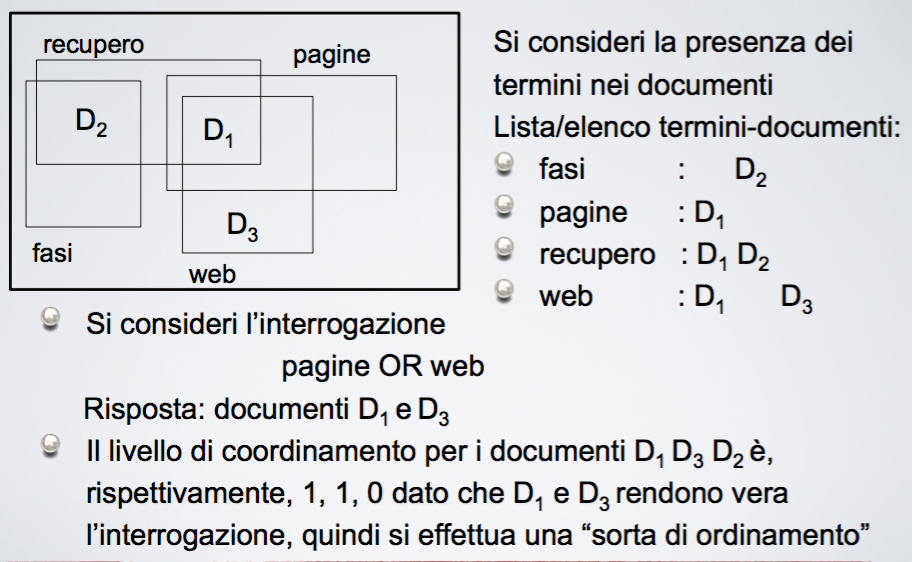
\includegraphics[width=0.7\linewidth]{images/l8-set-2}
		\caption{Livello di coordinamento con \textit{OR}}
	\end{minipage}
\end{figure}

\noindent Volendo si può uscire dalla logica booleana a due valori, introducendo un livello di coordinamento non binario, andando a considerare il numero di termini della query che sono in presenti nel documento.
Si può quindi utilizzare questo livello per ordinare i documenti forniti in risposta (a volte detto anche \textbf{simple matching}).

\textit{Questo vale solo con l'operatore AND}

Ad esempio si consideri l'interrogazione \textit{``pagine AND web''} per il nostro insieme di documenti.

Si può dire che l'interrogazione è ``più vera'' per D1, perché rende vere entrambe le proposizioni atomiche ``pagine'' e ``web'', che formano l'interrogazione, mentre D3 ne rende vera solo una e D2 nessuna.

\textbf{Piccola nota}: l'AND non è proprio un AND, è una sorta di AND-rilassato, perché un documento viene valutato positivamente anche un documento che non soddisfa tutti i termini.

\begin{figure}[htbp]
	\centering
	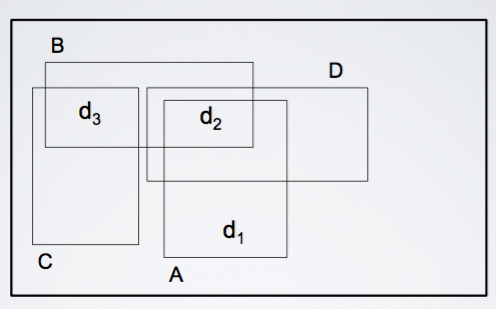
\includegraphics[width=0.7\linewidth]{images/l8-cord-gen}
	\caption{Livello di coordinamento non binario.}
\end{figure}

\subsection{Modello vettoriale}
%pacchetto slide 8

Questo modello assume che gli \textit{n} documenti e le interrogazioni appartengano ad uno spazio vettoriale composto da \textit{t} dimensioni, dove \textit{t} è il numero di dei termini indice (parole, frasi, \ldots).

Di conseguenza il documento $D_i$ è rappresentato da un vettore

$$
D_i = (d_{i,1},d_{i,2},\ldots,d_{i,j}, \ldots d_{i,t})
$$

\noindent dove l'elemento $d_{i,j}$ rappresenta il peso del termine $j$-esimo nel documento $i$-esimo.

Anche la query viene considerata come un documento. L'idea alla base di questo è che l'utente vorrebbe trovare un documento uguale alla query che sta scrivendo.

Una collezione di $n$ documenti può quindi essere rappresentata come una matrice dove ogni riga rappresenta un documento e ogni colonna contiene i pesi che sono associati ad un termine in un determinato documento.

\begin{figure}[htbp]
	\centering
	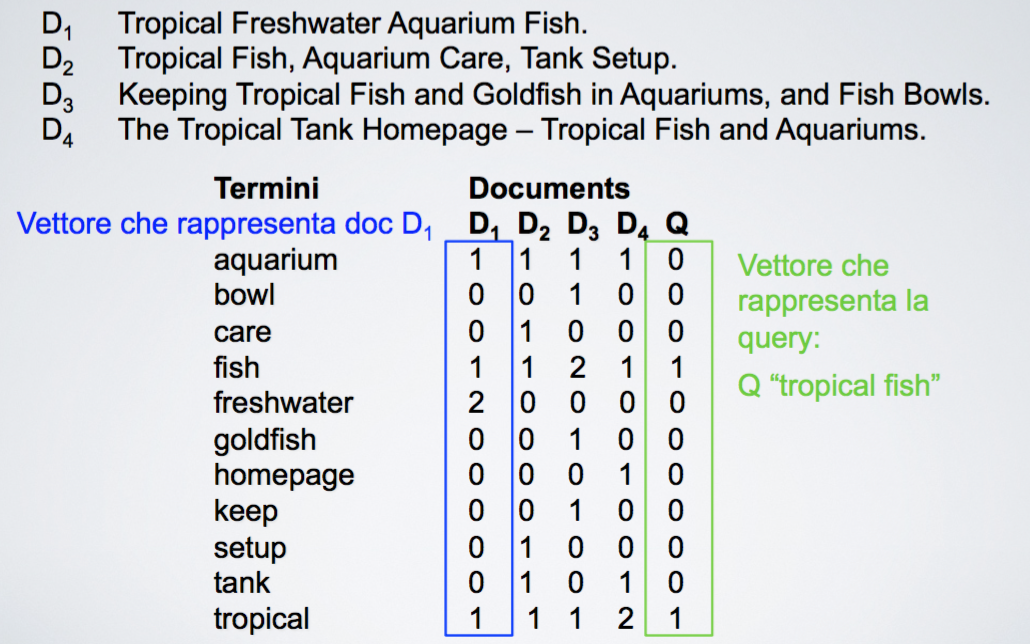
\includegraphics[width=0.5\linewidth]{images/l8-mod-vet}
	\caption{Nell'esempio viene utilizzato la frequenza della parola come peso del termine. Sono state inoltre rimosse le stop-word e viene fatto lo stemming dei plurali \textbf{NB:} la matrice riportata è trasposta rispetto a quella definita precedentemente.}
\end{figure}

\noindent Un'altra cosa carina del modello vettoriale è che in casi semplici può essere rappresentato in modo grafico.

\begin{figure}[htbp]
	\centering
	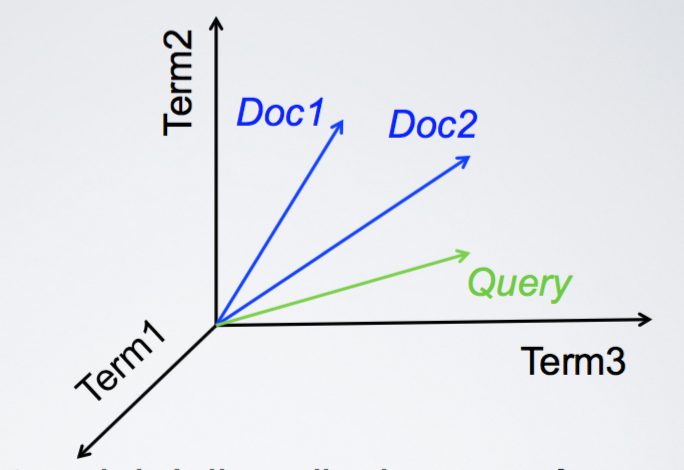
\includegraphics[width=0.5\linewidth]{images/l8-vet}
\end{figure}

\subsubsection{Metodo di ordinamento}

Data la rappresentazione vettoriale, i documenti possono essere riordinati utilizzando il risultato del calcolo della distanza fra il vettore di ciascuno documento e quello della query.

La distanza viene calcolata con una \textbf{misura di similarità} che ha un valore maggiore nel caso il documento sia simile alla query.
La misura più comune è la \textbf{cosine correlation} che calcola il coseno dell'angolo tra i due vettori.
La cosa interessante di questa misura è che quando i vettori sono normalizzati (hanno lunghezza uguale):

\begin{itemize}
	\item Il coseno dell'angolo $\alpha$ tra due vettori identici vale 1.
	\item Il coseno dell'angolo $\alpha$ tra due vettori che non condividono nessun termine o caratteristica vale 0.
\end{itemize} 

$$
Cosine(D_i, Q) = \frac{\sum\limits_j (d_{i,j} \cdot q_j)}{\sqrt{\sum\limits_j d_{i,j}^2 \cdot \sum\limits_j q_{j}^2}}
$$

\noindent con $j$ che varia da 1 a $t$.

\`E importante precisare che non ci sono ragioni teoriche che fanno preferire questa misura, si è semplicemente visto che funziona bene.

Ad esempio, per i documenti $D_1 = (0.5, 0.8, 0.3)$ e $D_2 = (0.9, 0.4, 0.2)$ e per la query $Q = (1.5, 1, 0)$ si ottengono le similarità:

\begin{align*}
	Cosine(D_1,Q) &= 0.87 \\
	Cosine(D_2, Q) &= 0.97
\end{align*}

\subsubsection{Pesatura dei termini}

Rimane comunque da definire degli schemi di pesatura per i vari termini.

La maggior parte degli schemi si basano sul \textbf{TF-IDF}, dove \textbf{TF} è la frequenza normalizzata del termine all'interno del documento:

$$
tf_{i,k} = \frac{f_{i,k}}{\sum\limits_j f_{i,j}}
$$

\noindent dove $k$ è il termine d'interesse, $f_{i,j}$ è la frequenza del termine $j$ nel documento $i$.

Tuttavia, così facendo viene dato molto peso ai termini molto frequenti nel documento e si è visto che a livello pratico utilizzare il logaritmo produce risultati migliori.

$$
tf_{i,k} = \frac{\log (f_{i,k}+1}{\sum\limits_j \log (f_{i,j} +1)}
$$
